\documentclass[11pt]{article}

\usepackage{hyperref}
\usepackage{amsmath}
\usepackage{enumerate}
\usepackage{tikz}
\usepackage{verbatim}
\usetikzlibrary{arrows}
\newcommand{\bigO}{\ensuremath{\mathcal{O}}}

\title{\textbf{Algoritmen en Complexiteit HW 4}}
\author{Jelte Fennema (10183159)\\
		Jaap Koetsier (10440615)\\
        Abe Wiersma (10433120)}
\date{6 maart 2014}

\begin{document}

\maketitle

\begin{enumerate}
    \item
        \begin{enumerate}
            \item
                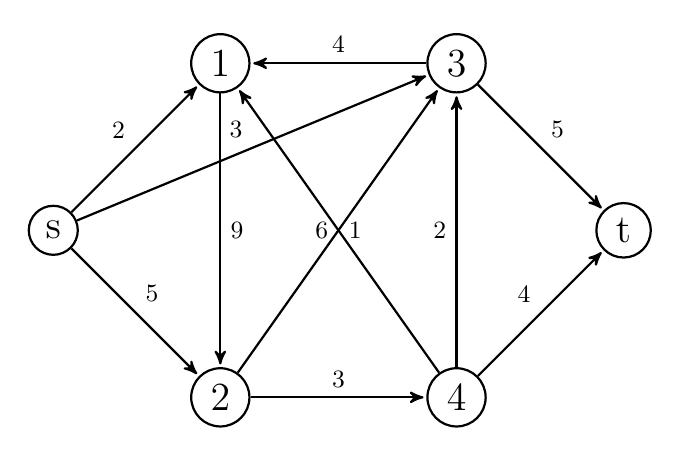
\begin{tikzpicture}[->,>=stealth',shorten >=1pt,auto,node distance=3cm,
                                    thick,main node/.style={circle,draw,font=\Large}]
                \node[main node] (S) {s};
                \node[main node] (1) [above right of=S] {1};
                \node[main node] (2) [below right of=S] {2};
                \node[main node] (3) [right of=1] {3};
                \node[main node] (4) [right of=2] {4};
                \node[main node] (T) [below right of=3] {t};
                \path[every node/.style={font=\small}]
                    (S) edge node {2} (1)
                        edge node {3} (3)
                        edge node {5} (2)
                    (1) edge node {9} (2)
                    (2) edge node [left] {6} (3)
                        edge node {3} (4)
                    (3) edge node [above] {4} (1)
                        edge node {5} (T)
                    (4) edge node {2} (3)
                        edge node {4} (T)
                        edge node [right] {1} (1);
                \end{tikzpicture}
            \item

            \item
            
        \end{enumerate}

    \item

    \item
        \begin{enumerate}
            \item

            \item

            \item

        \end{enumerate}

    \item

\end{enumerate}

\end{document}
